\documentclass{beamer}
\usetheme[hideothersubsections]{HRTheme}
\usepackage{beamerthemeHRTheme}
\usepackage{graphicx}
\usepackage[space]{grffile}
\usepackage{listings}
\lstset{language=C,
basicstyle=\ttfamily\footnotesize,
mathescape=true,
breaklines=true}
\usepackage[utf8]{inputenc}

\title{Computing machines architecture}

\author{The INFDEV Team @ HR}

\institute{Hogeschool Rotterdam \\ 
Rotterdam, Netherlands}

\date{}

\begin{document}
\maketitle

\SlideSection{Introduction}
\SlideSubSection{Lecture topics}
\begin{slide}{
\item We discuss the actual computational elements of a computer
\item We bridge what we have seen in the previous lecture with actual computer architectures
}\end{slide}

\SlideSection{Structure of a computer}
\SlideSubSection{Computational elements at a glance}
\begin{slide}{
\item CPU
\item Memory
}\end{slide}

\SlideSection{CPU and instructions}
\SlideSubSection{CPU}
\begin{slide}{
\item Read the current instruction from memory based on the \texttt{PC}
\item Evaluate the instruction
\begin{itemize}
\item Read and write memory elements as needed
\end{itemize}
\item Write the \texttt{PC} of the next instruction
}\end{slide}

\SlideSubSection{CPU instructions}
\begin{slide}{
\item \textit{Machine instructions}
\item Significantly smaller than what we use
\begin{itemize}
\item Register manipulation \texttt{add}, \texttt{sub}, \texttt{mul}, ...
\item Memory manipulation by integer address \texttt{lw}, \texttt{sw}
\end{itemize}
\item Concrete programming languages instructions equal many machine instructions
}\end{slide}

\SlideSubSection{Machine vs programming language instructions}
\begin{slide}{
\item There are different sorts of programming languages
\item Some higher level, some lower level
\item Lower level languages instructions equal few (even as low as one) machine instructions
\pause
\item Higher level languages instructions equal many (even as high as tens) machine instructions
}\end{slide}

\SlideSection{Memory and data}
\SlideSubSection{Memory}
\begin{slide}{
\item Data is stored into memory (and also the instructions).
\item Memory is just a long linear stream of bytes
\item CPU queries memory by address
\item CPU updates memory with address and data
}\end{slide}

\SlideSection{Memory and data}
\SlideSubSection{Different kinds of memory}
\begin{slide}{
\item There are two kinds of memory in a computer: Random Access Memory (RAM), and hard drives (HD).
\item RAM is volatile: the data is lost when the computer is powered off.
\item HD memory is permanent. Data remain after switching off the power.
\item The memory we are referring to in this lesson is the RAM.
}\end{slide}

\SlideSection{Memory and data}
\SlideSubSection{Different kinds of memory}
\begin{slide}{\item[] \begin{figure}
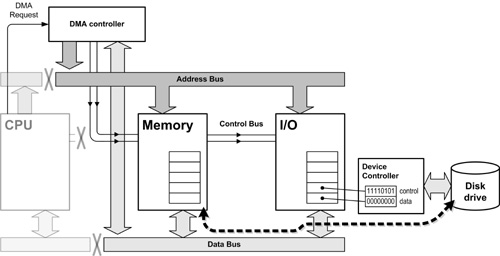
\includegraphics[scale=3.0]{../img/computer_architecture}
\caption{Architecture of a computer}.
\end{figure}}
\end{slide}

\SlideSection{Capabilities of programming languages}
\SlideSubSection{Typical programming language elements}
\begin{slide}{
\item Intuitive instruction structure
\item Higher level flow-control operators \\ \texttt{if, while, foreach, ...}
\item Labelled data through variables \\ \texttt{int studentAge = 19}
\item Higher level data manipulation operators \\ \texttt{hypotenuse = sqrt(x * x, y * y)}
}\end{slide}

\SlideSubSection{Instruction names}
\begin{slide}{
\item Machine instructions have names that are hard to pierce
\pause
\begin{itemize}
\item What is the meaning of instruction \texttt{0xDEBC318A}?
\pause
\item What is the meaning of instruction \texttt{currentUserAge := currentUserAge + 1}?
\end{itemize}
}\end{slide}

\SlideSubSection{Higher level flow-control operators}
\begin{slide}{
\item Machine instructions are tiny
\item Many standardized behaviors require lots of machine instructions
}\end{slide}

\begin{frame}[fragile]
Consider a \textit{fictional} machine language listing vs its high-level equivalent: \\ \ \\

\begin{tabular}{| c | c |}
\hline
\begin{lstlisting}
lw r1 r3
cmpi r0 r3 18
jmpsz ELSE
lw r4 r3
addi r3 r3 1 
sw r4 r3
jmp END
ELSE:
lw r5 r3
addi r3 r3 1 
sw r5 r3
END:
...
\end{lstlisting}

&

\begin{lstlisting}
if userAge >= 18 then
  adultUsers := adultUsers + 1
else
  youngUsers := youngUsers + 1  
...
\end{lstlisting}

\\
\hline
\end{tabular}
\end{frame}

\SlideSubSection{Variables}
\begin{slide}{
\item Program data is stored into variables
\item Variables \textit{label} memory data
\item \textit{Labels} simplify reasoning
\pause
\begin{itemize}
\item What is the meaning of \texttt{0xA0DF9931}?
\pause
\item What is the meaning of \texttt{userAge}?
\end{itemize}
}\end{slide}

\SlideSubSection{Variables and types}
\begin{slide}{
\item Program data in memory has no fixed structure
\item We can read 48 bytes instead of 32, and get 16 bytes of garbage for free
\item This causes errors
}\end{slide}

\begin{slide}{
\item Variables give a \textit{type} to memory data
\item \textit{Types} simplify reasoning
\pause
\begin{itemize}
\item How many bytes should I read at address \texttt{0xA0DF9931}?
\pause
\item How many bytes should I read for integer \texttt{userAge}\footnote{Knowing that integers are 4 bytes on 32 bit machines and 8 bytes on \\ 64 bit machines}?
\end{itemize}
}\end{slide}

\SlideSubSection{Yet more}
\begin{slide}{
\item Higher level programming languages do even more
\item Handle custom and complex computations (functions, events, continuations, lambda's)
\item Handle custom and complex data structures (structs, classes, tuples, ...)
}\end{slide}

%\item introduction to reasoning on post-conditions


\begin{frame}{This is it!}
\center
\fontsize{18pt}{7.2}\selectfont
The best of luck, and thanks for the attention!
\end{frame}

\end{document}

\begin{slide}{
\item ...
}\end{slide}

\begin{frame}[fragile]
\begin{lstlisting}
...
\end{lstlisting}
\end{frame}
